
% This LaTeX was auto-generated from an M-file by MATLAB.
% To make changes, update the M-file and republish this document.

\documentclass{article}
\usepackage{graphicx}
\usepackage{color}

\sloppy
\definecolor{lightgray}{gray}{0.5}
\setlength{\parindent}{0pt}

\begin{document}

    
    \begin{verbatim}
% first run prob7_3a b c d.m
clear
clc

nr=[-52:124];

syms n

% see table 5.2 page 392 oppenheim book
% to get X(jw) as 1 for 0<|w|<W and 0 else where
W=pi/2;
x1_n=(W/pi)*sinc(W/pi*n);

% note that x1 is defined for -52<=n<=124
x1=subs(x1_n,n,nr);

% to cover us for nan values
nan=find(isnan(x1));
x1(nan)=1;

N=2048;
wk=[0:N-1]*2*pi/N;

% note here fft was calculated for N=2048 hence it is defines
% N*ak for -52<=k<=-52+N-1
X1=fft(x1,N);

% test of fft and ifft
% since X1 define N*ak for -52<=k<=-52+2048 hence ifft should define x(n)
% for -52<=n<=-52+N-1
x1i=ifft(X1);

% note that X1i should be same as X1
X1i=fft(x1i,N);

figure(1)
clf

subplot(711)
plot(nr,x1);
title('nr against x1');

subplot(712)
plot(wk,abs(X1));
title('abs of X1 over wk for 0 to 2*pi but N*ak for -52<=k<=-52+N-1');

subplot(713)
plot(wk,unwrap(angle(X1)));
title('unwrapped angle for X1 over wk for 0 to 2*pi but N*ak for -52<=k<=-52+N-1');

subplot(714)
plot(wk,abs(X1i));
title('abs of X1i');

subplot(715)
plot(wk,unwrap(angle(X1i)));
title('unwrapped angle for X1i');

subplot(716)
plot([-52:-52+N-1],x1i); %careful here
title('ifft of X1 but over 2048 values starting from -52');

subplot(717)
plot(nr,x1i(1:length(x1))); %careful here
title('ifft of X1 but over only length of x1');

return
\end{verbatim}

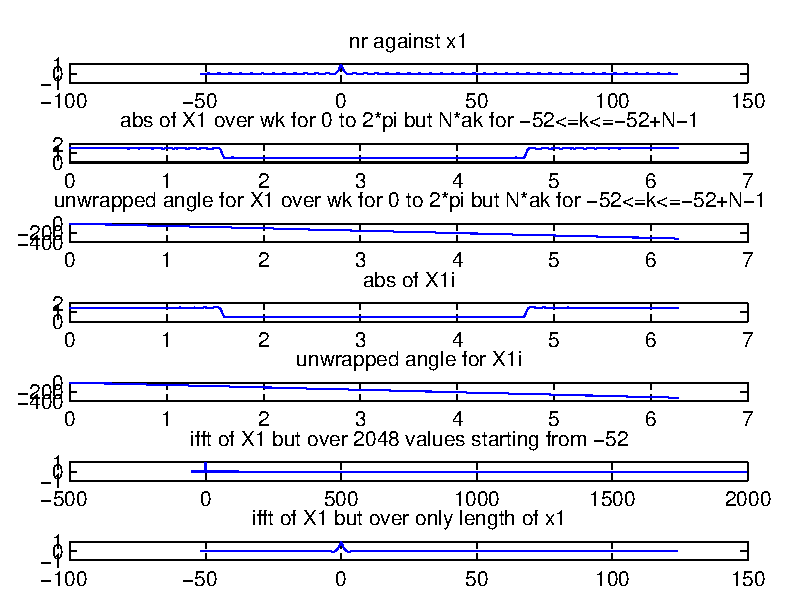
\includegraphics [width=4in]{prob7_3f_fft_ifft_test_01.eps}



\end{document}
    
